\section*{Einführung}
\subsection*{Algorithmische Mathematik -Was ist das?}
Gegenstand der Alma ist die Konstruktion und Analyse effizienter Algorithmen zur Lösung mathematischer Problemstellungen mit Hilfe des Computers. \\
Damit liegt sie im Bereich der Angewandten Mathematik. 
Konkrete Problemstellungen ergeben sich oft aus technischen Problemen, Naturwissenschaften, Medizin etc. \\
Man kann hierbei annehmen, dass verschiedene Problemstellungen aus der Anwendungen oft zu ähnlichen oder gleichen mathematischen Modellen zurückgeführt werden können. \\
Diese Probleme können wie folgt aussehen:
\begin{center}
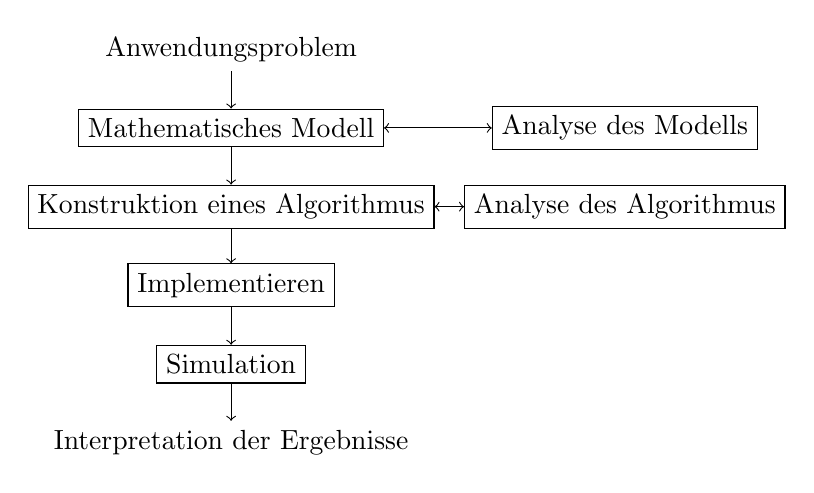
\begin{tikzpicture}
    \node(Anwendungsproblem) at (0,0) {Anwendungsproblem};
    \node[shape=rectangle,draw=black] (Mathematisches Modell) at (0,-1) {Mathematisches Modell};
    \node[shape=rectangle,draw=black] (Analyse des Modells) at (5,-1) {Analyse des Modells};
    \node[shape=rectangle,draw=black] (Konstruktion eines Algorithmus) at (0,-2) {Konstruktion eines Algorithmus};
    \node[shape=rectangle,draw=black] (Implementieren) at (0,-3){Implementieren};
    \node[shape=rectangle,draw=black] (Analyse des Algorithmus) at (5,-2){Analyse des Algorithmus};
    \node[shape=rectangle,draw=black] (Simulation) at (0,-4){Simulation};
    \node(Interpretation der Ergebnisse) at (0,-5){Interpretation der Ergebnisse};




    \path [->] (Anwendungsproblem) edge node {} (Mathematisches Modell);
    \path [->](Mathematisches Modell) edge node {} (Konstruktion eines Algorithmus);
    \path [->](Konstruktion eines Algorithmus) edge node {} (Implementieren);
    \path [->](Implementieren) edge node {} (Simulation);
    \path [->](Simulation) edge node {} (Interpretation der Ergebnisse);
    \path [<->](Mathematisches Modell) edge node {} (Analyse des Modells);
    \path [<->] (Konstruktion eines Algorithmus) edge node {} (Analyse des Algorithmus);
\end{tikzpicture}
\end{center}
\begin{example}
Ein typisches Problem ist das lösen eines linearen Gleichungssystems.
\end{example}
Im Rahmen dieser Vorlesung konzentrieren wird uns auf die Teilbereiche
\begin{enumerate}
	\item Numerik
	\item Diskrete Mathematik
	\item Statistik
\end{enumerate}
der Angewandten Mathematik
